% !TeX program = pdflatex
\documentclass[12pt,a4paper]{article}

% -------------------- Пакеты --------------------
% Вариант совместим с обычным pdfLaTeX в Overleaf.
% Не требует XeLaTeX/LuaLaTeX.
\usepackage{cmap}
\usepackage[T2A]{fontenc}
\usepackage[utf8]{inputenc}
\usepackage[english,russian]{babel}
\usepackage{tempora}

\usepackage[a4paper, left=20mm, right=20mm, top=20mm, bottom=20mm]{geometry}
\usepackage{amsmath, amssymb}
\usepackage{graphicx}
\usepackage{float}
\usepackage{booktabs}
\usepackage{array}
\usepackage{longtable}
\usepackage{tabularx}
\usepackage{multirow}
\usepackage{indentfirst}
\usepackage{titlesec}
\usepackage{caption}
\usepackage{subcaption}
\usepackage{hyperref}
\usepackage{xcolor}
\usepackage{listings}
\usepackage{microtype}

\hypersetup{
    colorlinks=true,
    linkcolor=black,
    urlcolor=blue,
    citecolor=black
}

\graphicspath{{figures_4.05/}}
\setlength{\parindent}{1.25cm}
\setlength{\parskip}{0.2em}
\titleformat{\section}{\normalfont\Large\bfseries}{\thesection}{1em}{}
\titleformat{\subsection}{\normalfont\large\bfseries}{\thesubsection}{1em}{}
\captionsetup{labelsep=period}

\newcommand{\um}{\ensuremath{\,\mu\text{м}}}
\newcommand{\nm}{\ensuremath{\,\text{нм}}}
\newcommand{\mm}{\ensuremath{\,\text{мм}}}
\newcommand{\Hz}{\ensuremath{\,\text{Гц}}}
\newcommand{\THz}{\ensuremath{\,\text{ТГц}}}
\newcommand{\fs}{\ensuremath{\,\text{фс}}}

\begin{document}

\begin{titlepage}
\begin{center}
Санкт-Петербургский национальный исследовательский институт\\
информационных технологий, механики и оптики

\vspace{3cm}

{\Large\bfseries ОТЧЁТ ПО ЛАБОРАТОРНОЙ РАБОТЕ №4.05}

\vspace{0.5cm}

{\large\bfseries «Изучение интерферометра Майкельсона»}

\vspace{2.5cm}
\end{center}

\begin{flushleft}
Группа: Z3244

Студенты:\\
Поминов Вадим\\
Забродский Александр\\
Фадеев Марк

Преподаватель:\\
Калантаевский Иван Эдуардович
\end{flushleft}

\vfill

\begin{flushleft}
К работе допущен:\\[0.4cm]
Работа выполнена:\\[0.4cm]
Отчет принят:
\end{flushleft}

\end{titlepage}

\section{Цель работы}

Изучение работы интерферометра Майкельсона и определение по интерференционной картине длины волны и ширины спектральной линии источника света.

\section{Задачи}

\begin{enumerate}
    \item Выполнить юстировку интерферометра Майкельсона.
    \item Экспериментально определить длину волны зеленой линии спектра ртутной лампы.
    \item Определить длину когерентности излучения по исчезновению интерференционной картины.
    \item Оценить время когерентности излучения.
    \item Оценить ширину спектральной линии источника света.
    \item Провести наблюдение интерференционной картины при использовании лазерного источника и объяснить полученный результат.
\end{enumerate}

\section{Объект исследования}

Объектом исследования является интерференционная картина, получаемая в интерферометре Майкельсона. В основной части работы используется излучение ртутной лампы, прошедшее через зеленый светофильтр. Дополнительно рассматривается картина, получаемая при освещении интерферометра лазером.

\section{Метод исследования}

В работе используется интерференция света методом деления амплитуды. Свет от источника делится светоделительной пластинкой на два пучка, которые проходят разные плечи интерферометра, отражаются от зеркал и затем снова складываются. Результат интерференции наблюдается на экране в виде полос равного наклона, имеющих форму концентрических колец.

При перемещении одного из зеркал микрометрическим винтом изменяется оптическая разность хода. Изменение положения зеркала приводит к появлению или исчезновению интерференционных колец. Подсчет числа прошедших колец позволяет определить длину волны излучения. Отдельно по положению, при котором интерференционная картина исчезает, оценивается длина когерентности.

\section{Рабочие формулы и исходные данные}

В центре интерференционной картины интенсивность может быть записана в виде
\begin{equation}
    I = I_0(1 + \cos k\Delta),
\end{equation}
где $I_0$ -- постоянный множитель, $k = 2\pi/\lambda$ -- волновое число, $\Delta$ -- оптическая разность хода.

Для интерферометра Майкельсона оптическая разность хода связана с разностью плеч выражением
\begin{equation}
    \Delta = 2|L_2 - L_1|.
\end{equation}
Если зеркало перемещается на расстояние $D$, то оптическая разность хода изменяется на величину $2D$. При изменении разности хода на одну длину волны через центр картины проходит одна интерференционная полоса. Поэтому длина волны определяется формулой
\begin{equation}
    \lambda = \frac{2D}{n},
    \label{eq:lambda}
\end{equation}
где $D = |d_2-d_1|$ -- перемещение зеркала, $n$ -- число появившихся или исчезнувших интерференционных колец.

Длина когерентности определяется по исчезновению интерференционной картины. Если при смещении зеркала на $D_{dis}$ кольца исчезают, то
\begin{equation}
    L_{\text{ког}} = 2D_{dis}.
    \label{eq:lcoh}
\end{equation}

Время когерентности связано с длиной когерентности выражением
\begin{equation}
    \tau_{\text{ког}} = \frac{L_{\text{ког}}}{c},
    \label{eq:tau}
\end{equation}
где $c = 2.998\cdot 10^8\,\text{м/с}$ -- скорость света.

Связь длины когерентности со спектральной шириной линии в приближенной оценке имеет вид
\begin{equation}
    L_{\text{ког}} \approx \frac{\lambda^2}{\Delta\lambda}.
\end{equation}
Отсюда ширина спектральной линии по длинам волн:
\begin{equation}
    \Delta\lambda = \frac{\lambda^2}{L_{\text{ког}}}.
    \label{eq:deltalambda}
\end{equation}

Частотная ширина линии оценивается по формуле
\begin{equation}
    \Delta\nu = \frac{c\Delta\lambda}{\lambda^2}.
    \label{eq:deltanu}
\end{equation}

В качестве табличного значения для зеленой линии ртути используется
\begin{equation}
    \lambda_{\text{табл}} = 546\nm.
\end{equation}

\section{Измерительные приборы}

\begin{table}[H]
\centering
\caption{Измерительные приборы и элементы установки}
\begin{tabularx}{\textwidth}{>{\raggedright\arraybackslash}X>{\raggedright\arraybackslash}X>{\raggedright\arraybackslash}X}
\toprule
Наименование & Назначение & Особенности использования \\
\midrule
Интерферометр Майкельсона & Получение интерференционной картины & Используются два зеркала и светоделительная пластинка \\
Микрометрический винт & Перемещение зеркала $M_2$ & По изменению отсчета определяется смещение зеркала \\
Ртутная лампа & Источник немонохроматического света & Используется вместе с зеленым светофильтром \\
Зеленый светофильтр & Выделение зеленой области спектра & Для сравнения используется линия ртути $546\nm$ \\
Лазер & Источник квазимонохроматического излучения & Используется для дополнительного наблюдения картины \\
Экран & Наблюдение интерференционной картины & На экране наблюдаются кольца равного наклона \\
\bottomrule
\end{tabularx}
\end{table}

\section{Проведение измерений}

Сначала была выполнена настройка установки с ртутной лампой. Свет от лампы проходил через ирисовую диафрагму, линзу и зеленый светофильтр, после чего попадал в интерферометр Майкельсона. С помощью юстировочных винтов зеркала $M_1$ добивались совмещения двух изображений и появления интерференционной картины в виде колец.

Для определения длины волны фиксировались начальный и конечный отсчеты по микрометрическому винту $d_1$ и $d_2$, а также число наблюдаемых темных колец. По условию работы можно считать либо светлые, либо темные кольца; в данной работе обрабатывалась одна и та же система темных колец.

Для определения длины когерентности зеркало устанавливали около положения нулевой разности хода. Затем микрометрический винт вращали в одну и в другую сторону до положения, при котором интерференционные кольца исчезали. В таблицу заносились положения исчезновения картины.

После этого использовался лазерный источник. При изменении положения зеркала заметного изменения числа колец и исчезновения картины в доступном диапазоне перемещения не наблюдалось.

\section{Результаты прямых измерений и первичная обработка}

\subsection{Измерения для определения длины волны}

В таблице \ref{tab:lambda_raw} приведены результаты серии измерений для ртутной лампы с зеленым фильтром. Первая строка соответствует начальному состоянию при $d_1=d_2=4\um$, поэтому $D=0$ и эта строка не используется при вычислении среднего значения длины волны по формуле \eqref{eq:lambda}.

\begin{table}[H]
\centering
\caption{Результаты измерений для определения длины волны}
\label{tab:lambda_raw}
\begin{tabular}{cccccc}
\toprule
$N$ & $d_1$, мкм & $d_2$, мкм & $D$, мкм & $n$, шт & $\lambda_N$, нм \\
\midrule
1 & 4.00 & 4.00 & 0.00 & 17 & -- \\
2 & 4.00 & 4.05 & 0.05 & 16 & 6.25 \\
3 & 4.00 & 4.10 & 0.10 & 16 & 12.50 \\
4 & 4.00 & 4.15 & 0.15 & 15 & 20.00 \\
5 & 4.00 & 4.20 & 0.20 & 14 & 28.57 \\
\bottomrule
\end{tabular}
\end{table}

Вычислим среднее значение по строкам 2--5:
\begin{equation}
    \overline{\lambda}_{\text{эксп}} = \frac{6.25+12.50+20.00+28.57}{4}=16.83\nm.
\end{equation}

Среднеквадратичное отклонение по серии:
\begin{equation}
    s_\lambda = \sqrt{\frac{\sum\limits_{i=1}^{4}(\lambda_i-\overline{\lambda})^2}{4-1}} \approx 9.63\nm.
\end{equation}

Для доверительной вероятности $P=0.95$ и числа степеней свободы $f=3$ принимаем $t_{0.95;3}=3.182$. Тогда доверительная погрешность среднего:
\begin{equation}
    \Delta\lambda_{\text{разб}} = t_{0.95;3}\frac{s_\lambda}{\sqrt{4}} \approx 15.33\nm.
\end{equation}

Получается
\begin{equation}
    \lambda_{\text{эксп}} = (16.83 \pm 15.33)\nm.
\end{equation}

Это значение сильно отличается от табличного значения зеленой линии ртути $546\nm$. Относительное расхождение:
\begin{equation}
    \delta = \frac{|546-16.83|}{546}\cdot 100\% \approx 96.9\%.
\end{equation}

Такое расхождение не может объясняться только приборной погрешностью. Наиболее вероятная причина состоит в том, что в журнале была записана не серия корректных интервальных измерений числа прошедших полос, а число наблюдаемых колец в текущем положении зеркала. Поэтому данная серия используется в отчете как демонстрация обработки по формуле \eqref{eq:lambda}, но для дальнейшей оценки ширины спектральной линии используется физически корректное табличное значение $\lambda_{\text{табл}}=546\nm$.

\begin{figure}[H]
\centering
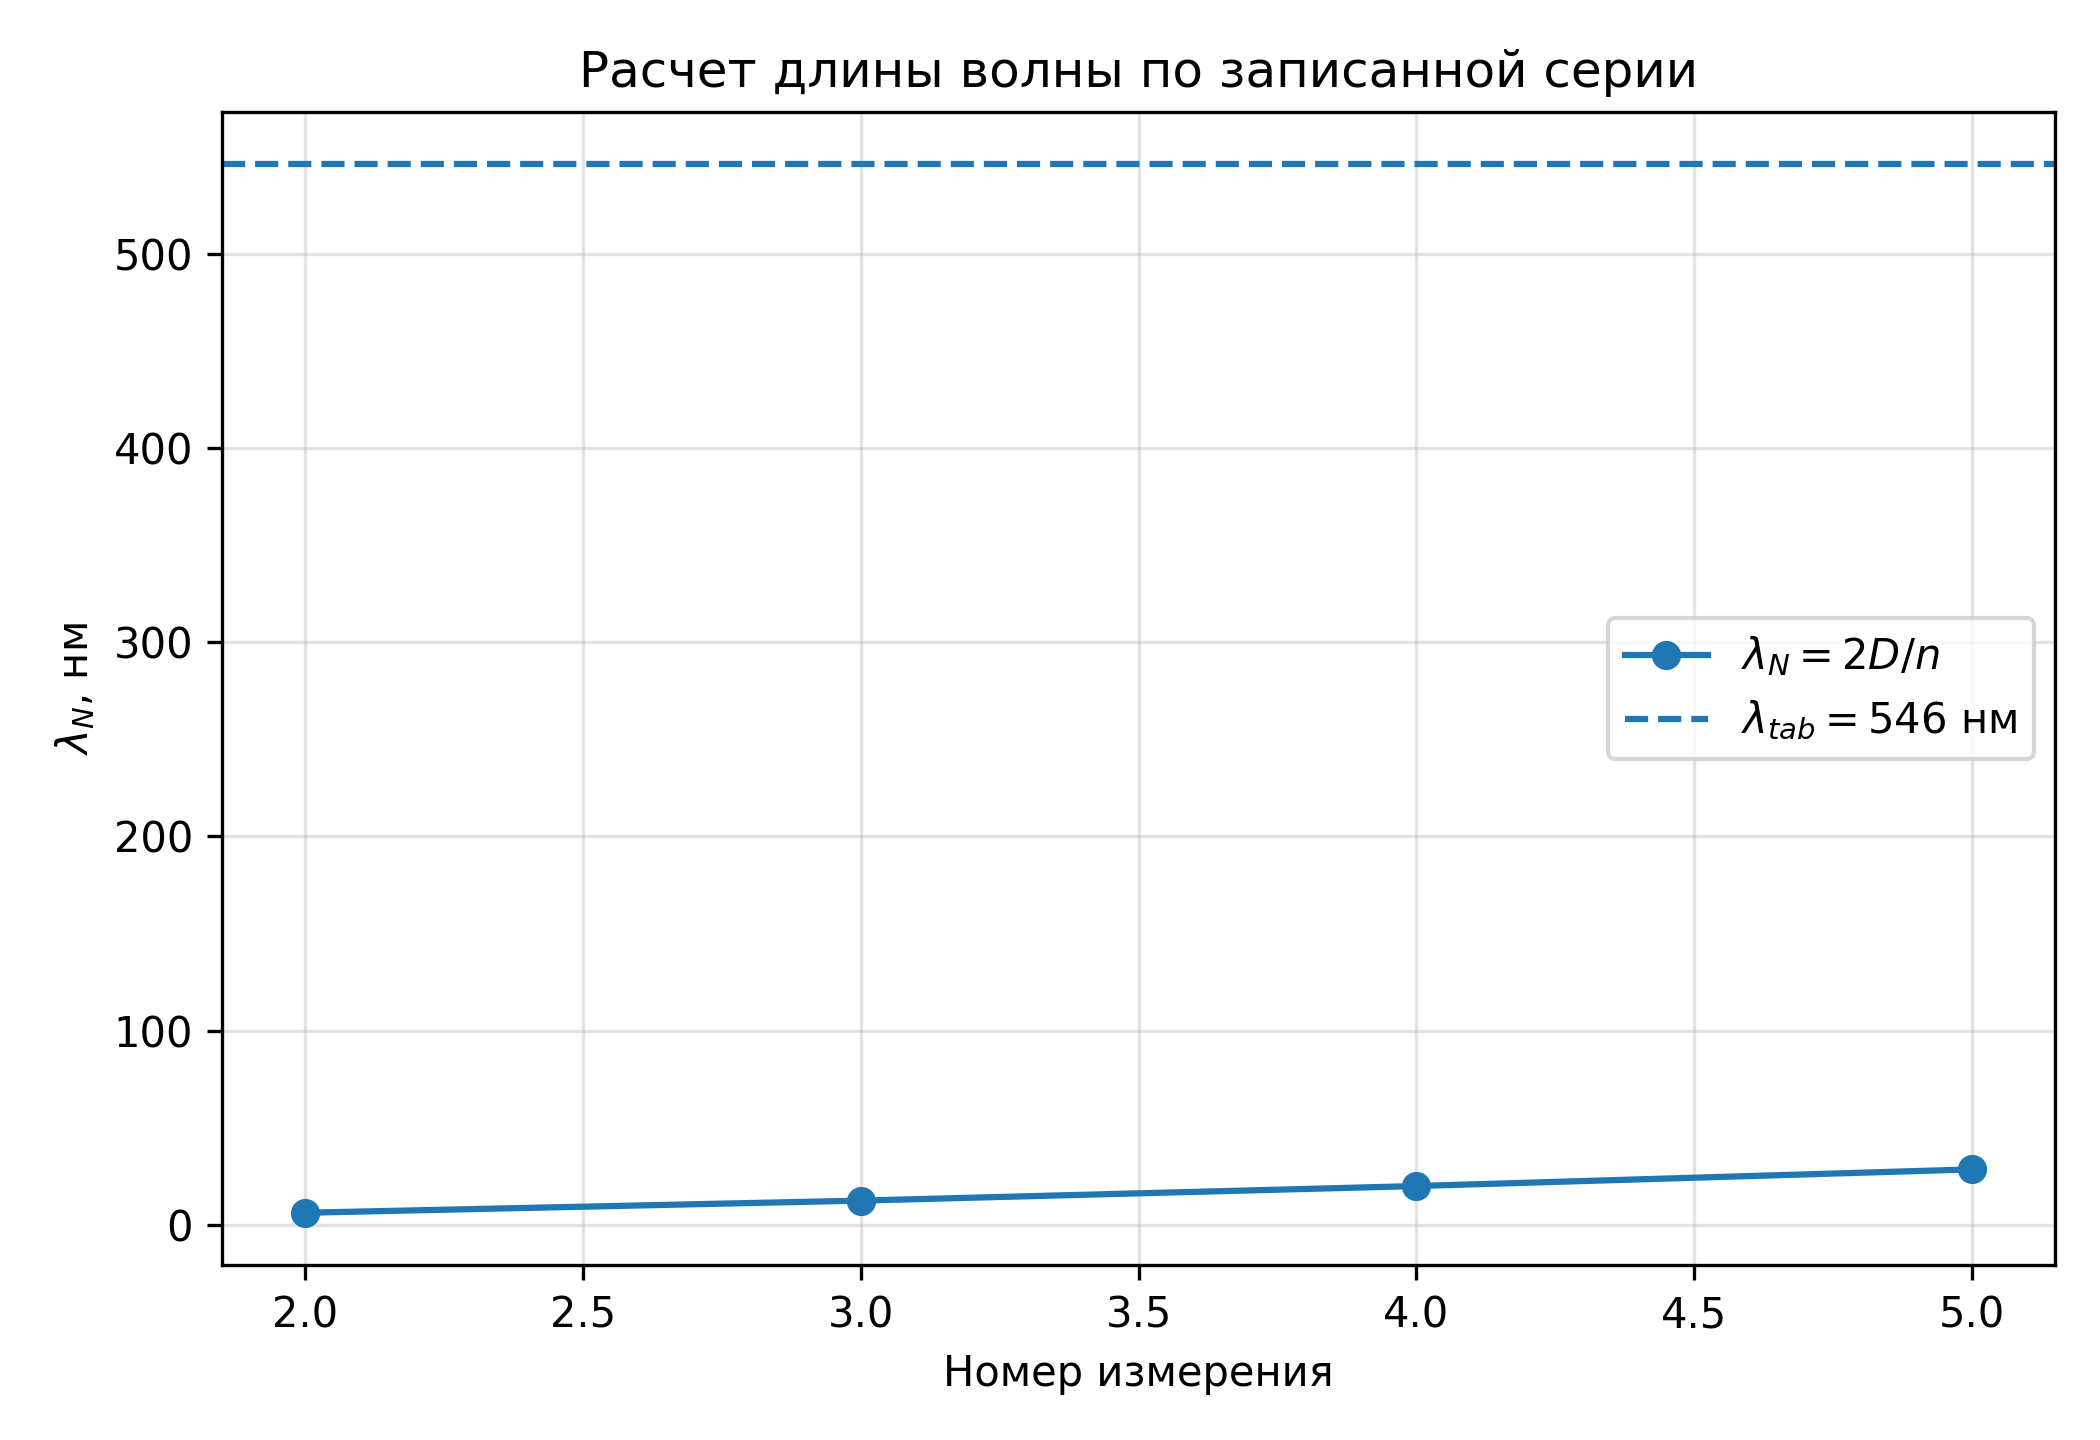
\includegraphics[width=0.78\textwidth]{wavelength_raw.png}
\caption{Значения длины волны, полученные по записанной серии измерений. Пунктиром показано табличное значение зеленой линии ртути.}
\end{figure}

\subsection{Измерения для определения длины когерентности}

В таблице \ref{tab:coherence} приведены положения исчезновения интерференционной картины. За положение нулевой разности хода по записи измерений принимаем
\begin{equation}
    d_0 = 4.00\um.
\end{equation}
Смещение зеркала рассчитывается как
\begin{equation}
    D = |d_{dis}-d_0|,
\end{equation}
а длина когерентности -- по формуле \eqref{eq:lcoh}.

\begin{table}[H]
\centering
\caption{Оценка длины когерентности по исчезновению интерференционной картины}
\label{tab:coherence}
\begin{tabular}{ccccc}
\toprule
Направление вращения & $N$ & $d_{dis}$, мкм & $D$, мкм & $L_{\text{ког}}$, мкм \\
\midrule
В большую сторону & 1 & 5.80 & 1.80 & 3.60 \\
В большую сторону & 2 & 5.90 & 1.90 & 3.80 \\
В большую сторону & 3 & 6.00 & 2.00 & 4.00 \\
В меньшую сторону & 1 & 3.15 & 0.85 & 1.70 \\
В меньшую сторону & 2 & 1.50 & 2.50 & 5.00 \\
В меньшую сторону & 3 & 1.70 & 2.30 & 4.60 \\
\bottomrule
\end{tabular}
\end{table}

Средняя длина когерентности:
\begin{equation}
    \overline{L}_{\text{ког}} = \frac{3.60+3.80+4.00+1.70+5.00+4.60}{6}=3.78\um.
\end{equation}

Среднеквадратичное отклонение:
\begin{equation}
    s_L = \sqrt{\frac{\sum\limits_{i=1}^{6}(L_i-\overline{L})^2}{6-1}} \approx 1.15\um.
\end{equation}

Для $P=0.95$ и $f=5$ принимаем $t_{0.95;5}=2.571$. Тогда доверительная погрешность среднего:
\begin{equation}
    \Delta L_{\text{ког}} = t_{0.95;5}\frac{s_L}{\sqrt{6}} \approx 1.20\um.
\end{equation}

Итак,
\begin{equation}
    L_{\text{ког}} = (3.78 \pm 1.20)\um.
\end{equation}

\begin{figure}[H]
\centering
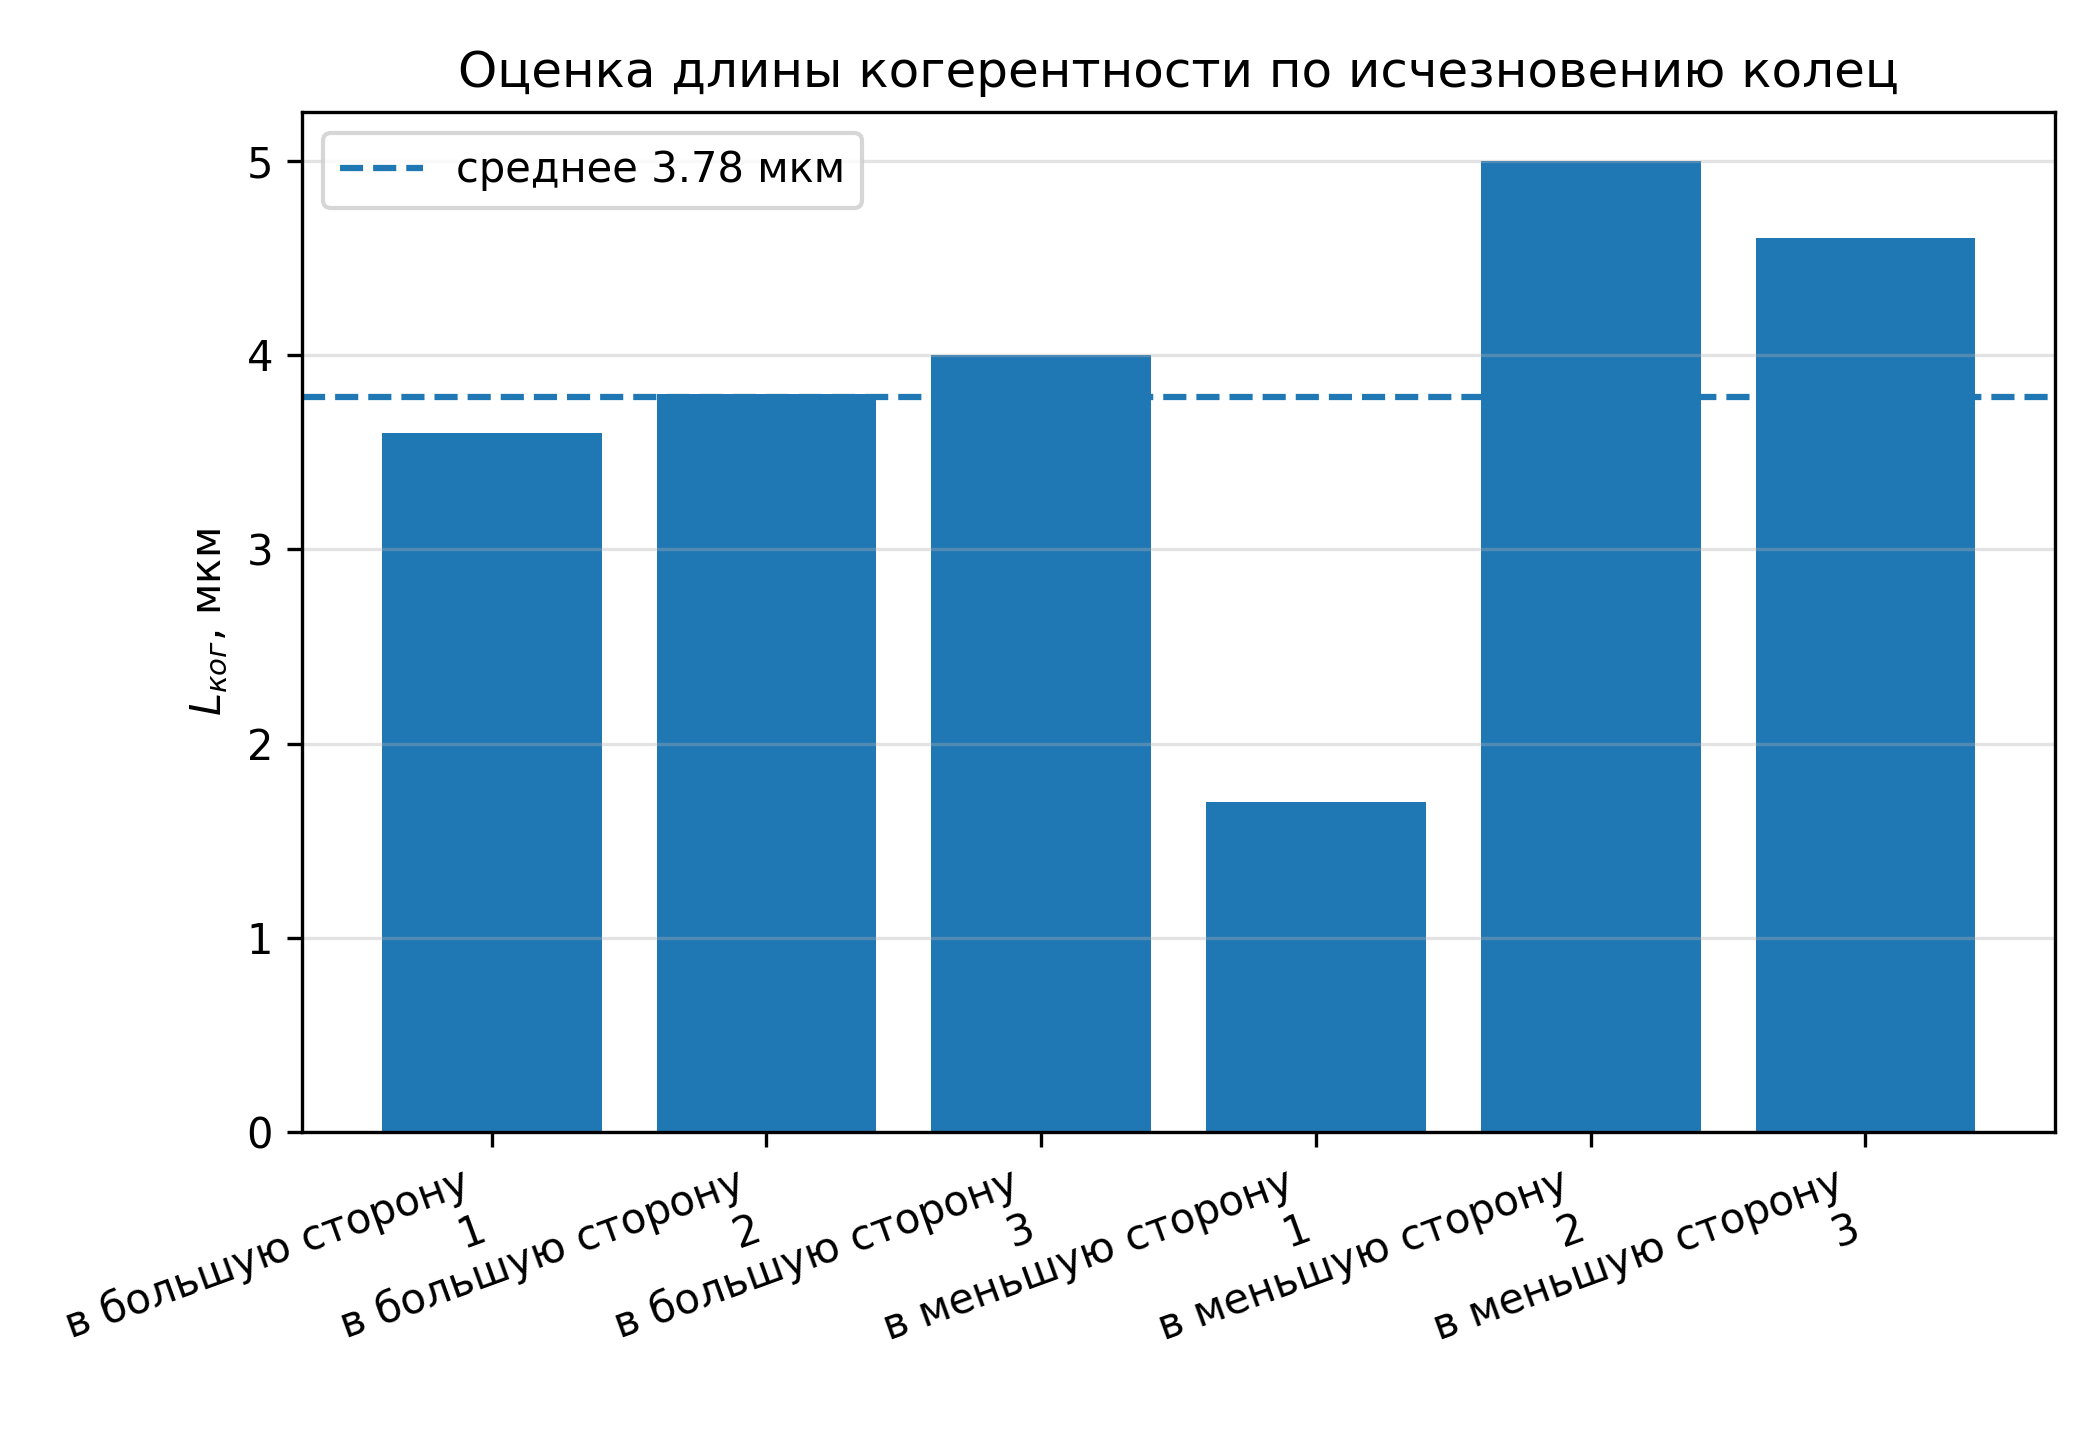
\includegraphics[width=0.82\textwidth]{coherence_length.png}
\caption{Значения длины когерентности, найденные по положениям исчезновения интерференционной картины.}
\end{figure}

\section{Расчет косвенных величин}

\subsection{Время когерентности}

Переведем длину когерентности в метры:
\begin{equation}
    L_{\text{ког}} = 3.78\um = 3.78\cdot 10^{-6}\text{ м}.
\end{equation}

По формуле \eqref{eq:tau} получаем
\begin{equation}
    \tau_{\text{ког}} = \frac{3.78\cdot 10^{-6}}{2.998\cdot 10^8}
    \approx 1.26\cdot 10^{-14}\text{ с}.
\end{equation}

В фемтосекундах:
\begin{equation}
    \tau_{\text{ког}} \approx 12.62\fs.
\end{equation}

Относительная погрешность времени когерентности равна относительной погрешности длины когерентности:
\begin{equation}
    \frac{\Delta\tau}{\tau}=\frac{\Delta L}{L}=\frac{1.20}{3.78}\approx 0.318.
\end{equation}
Следовательно,
\begin{equation}
    \Delta\tau \approx 12.62\cdot 0.318 \approx 4.01\fs.
\end{equation}
Итог:
\begin{equation}
    \tau_{\text{ког}} = (12.6 \pm 4.0)\fs.
\end{equation}

\subsection{Ширина спектральной линии по длинам волн}

Так как экспериментальная серия для определения $\lambda$ записана некорректно для количественного определения длины волны, для оценки ширины спектральной линии используем табличное значение зеленой линии ртути:
\begin{equation}
    \lambda = 546\nm.
\end{equation}

Переведем длину когерентности в нанометры:
\begin{equation}
    L_{\text{ког}} = 3.78\um = 3783\nm.
\end{equation}

По формуле \eqref{eq:deltalambda}:
\begin{equation}
    \Delta\lambda = \frac{546^2}{3783} \approx 78.8\nm.
\end{equation}

Так как $\Delta\lambda \sim 1/L_{\text{ког}}$, относительная погрешность ширины линии равна относительной погрешности длины когерентности:
\begin{equation}
    \frac{\Delta(\Delta\lambda)}{\Delta\lambda}=\frac{\Delta L_{\text{ког}}}{L_{\text{ког}}}=\frac{1.20}{3.78}\approx 0.318.
\end{equation}

Тогда
\begin{equation}
    \Delta(\Delta\lambda) \approx 78.8\cdot 0.318 \approx 25.1\nm.
\end{equation}

Итог:
\begin{equation}
    \Delta\lambda = (78.8 \pm 25.1)\nm.
\end{equation}

\subsection{Ширина спектральной линии по частоте}

По формуле \eqref{eq:deltanu}:
\begin{equation}
    \Delta\nu = \frac{c\Delta\lambda}{\lambda^2}.
\end{equation}

Подставим значения в СИ:
\begin{equation}
    \lambda = 546\cdot 10^{-9}\text{ м}, \qquad
    \Delta\lambda = 78.8\cdot 10^{-9}\text{ м}.
\end{equation}

Тогда
\begin{equation}
    \Delta\nu = \frac{2.998\cdot 10^8\cdot 78.8\cdot 10^{-9}}{(546\cdot 10^{-9})^2}
    \approx 7.92\cdot 10^{13}\Hz.
\end{equation}

В терагерцах:
\begin{equation}
    \Delta\nu \approx 79.2\THz.
\end{equation}

Погрешность:
\begin{equation}
    \Delta(\Delta\nu) \approx 25.2\THz.
\end{equation}

Итог:
\begin{equation}
    \Delta\nu = (79.2 \pm 25.2)\THz.
\end{equation}

\section{Наблюдение с лазером}

В отдельной серии измерений использовался лазерный источник. Результаты наблюдения приведены в таблице \ref{tab:laser}. В журнале измерений указано, что при изменении положения микрометрического винта число наблюдаемых колец не менялось.

\begin{table}[H]
\centering
\caption{Наблюдение интерференционной картины при использовании лазера}
\label{tab:laser}
\begin{tabular}{ccccc}
\toprule
$N$ & $d_1$, мкм & $d_2$, мкм & $D$, мкм & Число колец \\
\midrule
1 & 4.00 & 4.00 & 0.00 & 13 \\
2 & 4.00 & 4.05 & 0.05 & 13 \\
3 & 4.00 & 5.60 & 1.60 & 13 \\
\bottomrule
\end{tabular}
\end{table}

Максимальное изменение оптической разности хода в этой серии:
\begin{equation}
    \Delta_{\max}=2D_{\max}=2\cdot 1.60=3.20\um.
\end{equation}

Интерференционная картина не исчезла даже при таком изменении разности хода. Следовательно, для данной серии можно записать нижнюю оценку:
\begin{equation}
    L_{\text{ког, лазер}} > 3.20\um.
\end{equation}

Это ожидаемый результат. Лазерное излучение имеет значительно меньшую спектральную ширину и, следовательно, большую длину когерентности по сравнению с излучением ртутной лампы после светофильтра. Поэтому в доступном диапазоне перемещения зеркала интерференционная картина не исчезает. По этой причине оценить ширину спектральной линии лазера данным способом на используемой установке невозможно: доступная разность хода слишком мала по сравнению с длиной когерентности лазерного источника.

\begin{figure}[H]
\centering
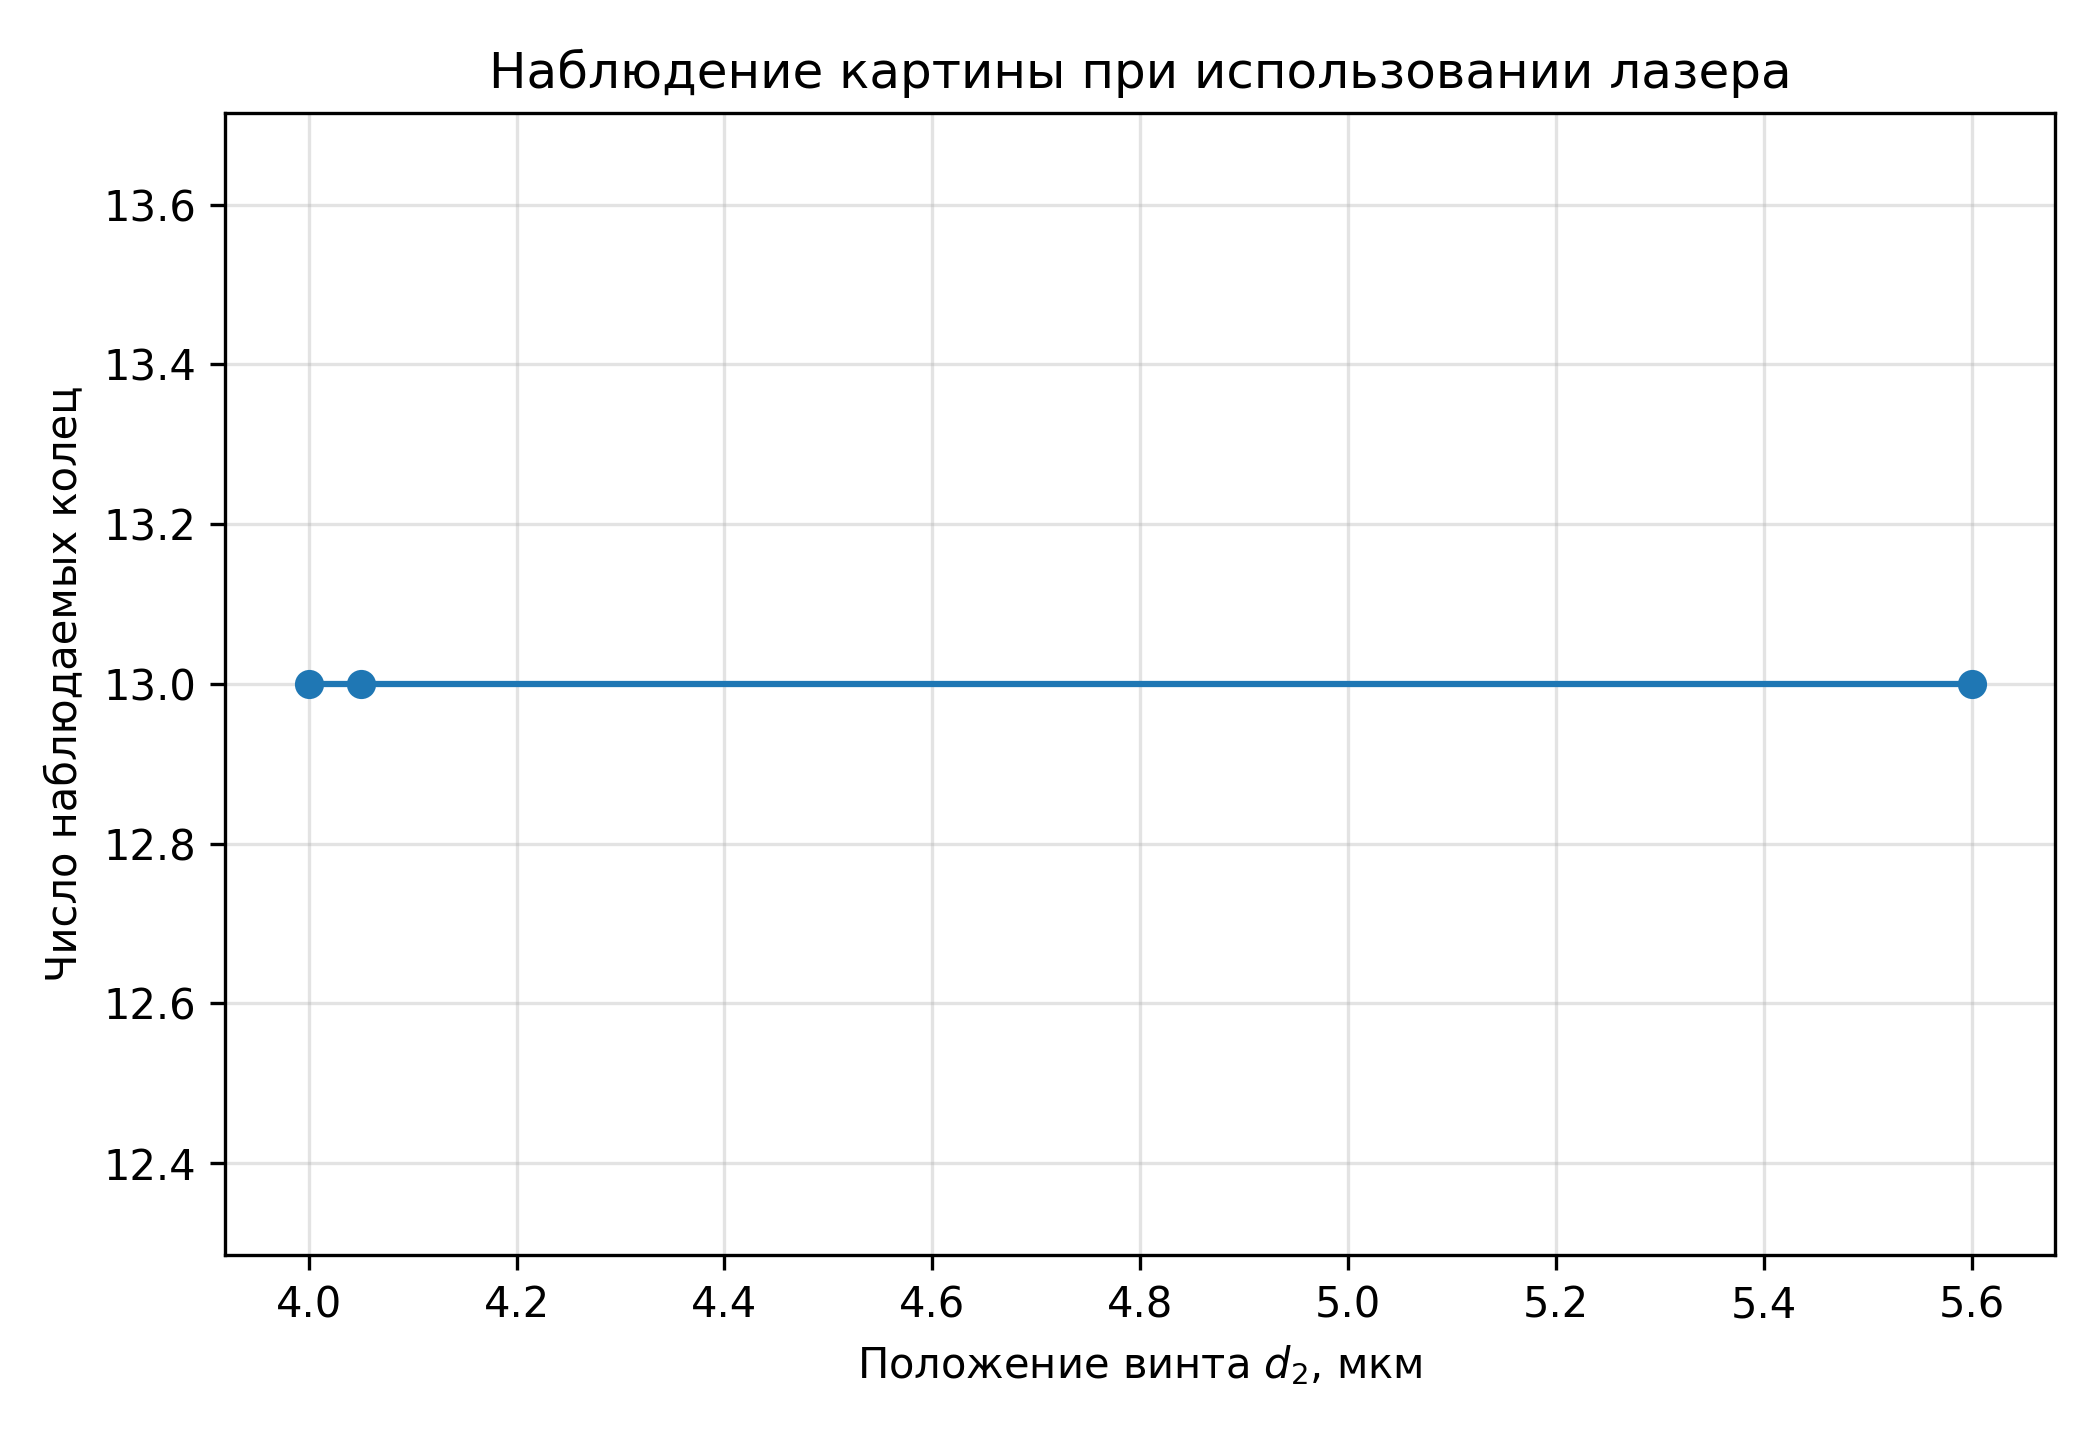
\includegraphics[width=0.78\textwidth]{laser_observation.png}
\caption{При использовании лазера число наблюдаемых колец в записанной серии практически не изменялось.}
\end{figure}

\section{Оценка погрешностей}

Основной вклад в погрешность определения длины волны по формуле \eqref{eq:lambda} вносит не приборная погрешность микрометрического винта, а неточность визуального подсчета колец и малая величина перемещения зеркала. По записанной серии разброс полученных значений длины волны оказался настолько большим, что результат нельзя считать физически корректным.

Для длины когерентности погрешность оценивалась по разбросу шести измерений:
\begin{equation}
    \Delta L_{\text{ког}} = t_{0.95;5}\frac{s_L}{\sqrt{6}} = 1.20\um.
\end{equation}

Погрешности времени когерентности и ширины спектральной линии определялись через относительную погрешность длины когерентности:
\begin{equation}
    \frac{\Delta\tau}{\tau}=\frac{\Delta L_{\text{ког}}}{L_{\text{ког}}},
    \qquad
    \frac{\Delta(\Delta\lambda)}{\Delta\lambda}=\frac{\Delta L_{\text{ког}}}{L_{\text{ког}}}.
\end{equation}

\section{Окончательные результаты}

\begin{table}[H]
\centering
\caption{Итоговые результаты работы}
\begin{tabularx}{\textwidth}{>{\raggedright\arraybackslash}X>{\centering\arraybackslash}X}
\toprule
Величина & Значение \\
\midrule
Длина волны по записанной серии & $(16.8 \pm 15.3)\nm$ \\
Табличная длина волны зеленой линии ртути & $546\nm$ \\
Длина когерентности ртутной лампы с фильтром & $(3.78 \pm 1.20)\um$ \\
Время когерентности & $(12.6 \pm 4.0)\fs$ \\
Ширина спектральной линии по длинам волн & $(78.8 \pm 25.1)\nm$ \\
Ширина спектральной линии по частоте & $(79.2 \pm 25.2)\THz$ \\
Нижняя оценка длины когерентности лазера & $L_{\text{ког, лазер}}>3.20\um$ \\
\bottomrule
\end{tabularx}
\end{table}

\section{Выводы и анализ результатов работы}

В ходе лабораторной работы была изучена работа интерферометра Майкельсона. При освещении установки ртутной лампой с зеленым светофильтром наблюдалась интерференционная картина в виде концентрических колец равного наклона.

По записанной серии измерений была выполнена обработка для определения длины волны по формуле $\lambda=2D/n$. Полученное значение $(16.8\pm 15.3)\nm$ резко отличается от табличного значения $546\nm$. Это указывает на ошибку в записи или интерпретации числа колец: вероятнее всего, в таблицу было занесено число наблюдаемых колец в текущем положении, а не число колец, прошедших через центр за интервал перемещения зеркала. Поэтому этот результат не используется как достоверное значение длины волны.

По исчезновению интерференционной картины была оценена длина когерентности излучения ртутной лампы с зеленым фильтром:
\begin{equation}
    L_{\text{ког}}=(3.78\pm 1.20)\um.
\end{equation}
Соответствующее время когерентности составило
\begin{equation}
    \tau_{\text{ког}}=(12.6\pm 4.0)\fs.
\end{equation}
По этим данным была получена оценка ширины спектральной линии:
\begin{equation}
    \Delta\lambda=(78.8\pm 25.1)\nm.
\end{equation}

При использовании лазера число наблюдаемых колец в доступном диапазоне перемещения зеркала не изменялось, а исчезновения интерференционной картины не наблюдалось. Это объясняется значительно большей длиной когерентности лазерного излучения. Поэтому для лазера в данной работе можно дать только нижнюю оценку длины когерентности: $L_{\text{ког, лазер}}>3.20\um$.

\end{document}
